\documentclass{article}
\usepackage[utf8]{inputenc}

\title{Physics 242 Final Assignment\\Invidual Report}
\author{Xiaojian Jin}
\date{June 10, 2016}
\usepackage{amsmath,amsthm,amssymb, graphicx, multicol, array,mathrsfs,listings}
\usepackage[export]{adjustbox}
\begin{document}

\maketitle

In this final project, my group with myself had to simulate stock price and price Asian option with MCMC.\\
My job is :\\
\begin{enumerate}
\item to provide background financial knowledge for my partners, such as explanation of Asian options and Black-Scholes model.
\item to design 4-step algorithm to price the option.
\begin{enumerate}
\item averaging the stock price for each of the simulated paths.
\item applying the appropriate formula of (1) and (2).
\item averaging the payoffs for all paths.
\item discounting the result back to current price.
\end{enumerate}
\item to derive the risky asset equation by the geometric Brownian motion and the Ito equations.
\item to study how to implement Metropolis-adjusted Langevin algorithm into our simulation with my partners. We figured out the transition probability density and probability density for accepting or rejecting the proposal path.
\item to code the toy model to test the correctness of our analysis and provide it for my partners to design the CUDA code. The image above is generate from my toy model:\\
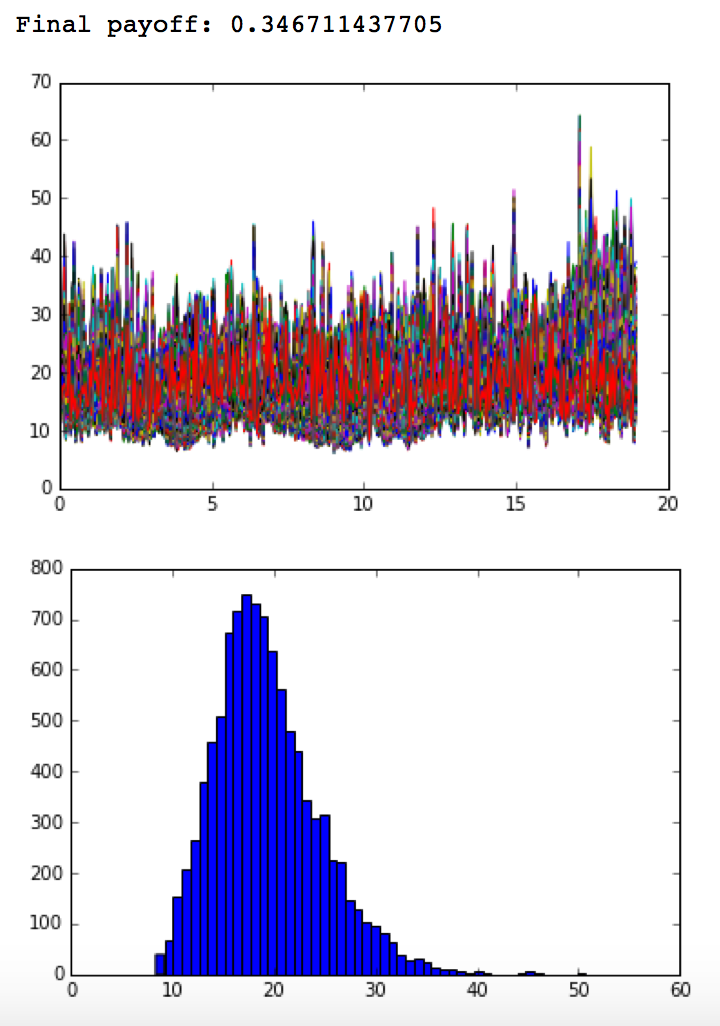
\includegraphics[scale=0.3,center]{toymodel}

\end{enumerate}
From this project, I learned how to develop simulation through the Monte Carlo methods with the Metropolis method. This also deepened my understanding on equity options.


\end{document}
